\pdfminorversion=7
\ifdefined\MakeCleanCopy
\documentclass[sigconf,anonymous,nonacm]{acmart}
\else
\documentclass[sigconf,anonymous,review,nonacm]{acmart}
\fi

% Packages used by the manuscript. The ACM class supplies the conference
% typography, hyperlinks, and standard color support.
\usepackage{booktabs}
\usepackage{graphicx}
\usepackage{microtype}
\AtBeginDocument{\raggedbottom}
% Red identifies revised or added prose, tables, and captions.
% Change \revisionstrue to \revisionsfalse for a clean reading copy.
\newif\ifrevisions
\ifdefined\MakeCleanCopy\revisionsfalse\else\revisionstrue\fi
\newcommand{\rev}[1]{\ifrevisions\textcolor{red}{#1}\else#1\fi}
\newenvironment{revblock}{\begingroup\ifrevisions\color{red}\fi}{\endgroup}
% This is a review copy, without fictitious publication metadata.
\setcopyright{none}
\settopmatter{printacmref=false}
\acmDOI{}
\acmISBN{}
\usepackage{placeins}
\pdfstringdefDisableCommands{\def\rev#1{#1}}
% Mark the newly added reference; existing entries remain black.
\AtBeginEnvironment{thebibliography}{%
  \let\originalbibitem\bibitem
  \renewcommand{\bibitem}[2][]{%
    \ifstrequal{#2}{teinemaa2019outcome}{\ifrevisions\color{red}\fi}{\color{black}}%
    \originalbibitem[#1]{#2}}}

\usepackage{float}
\usepackage{balance}
\makeatletter\@ACM@balancefalse\makeatother
\definecolor{logicbg}{HTML}{EDF6F3}
\newcommand{\vse}[2]{\ensuremath{#1\!{\scriptstyle\,\pm\,#2}}}
\newcommand{\bse}[2]{\ensuremath{\mathbf{#1}\!{\scriptstyle\,\pm\,#2}}}
\setlength{\textfloatsep}{9pt plus 1pt minus 1pt}
\setlength{\dbltextfloatsep}{9pt plus 1pt minus 1pt}
\setlength{\floatsep}{7pt plus 1pt minus 1pt}
\setlength{\dblfloatsep}{7pt plus 1pt minus 1pt}
\renewcommand{\topfraction}{0.95}
\renewcommand{\dbltopfraction}{0.95}
\renewcommand{\textfraction}{0.05}

\usepackage{tikz}
\usepackage{bbm}
\usepackage{multirow}
\usepackage{amsmath}
\usepackage{tabularx} % 請確保 preamble 有引進 tabularx 與 booktabs
\usepackage{booktabs}

\usetikzlibrary{arrows.meta,calc,decorations.pathreplacing}

% Show a placeholder until the corresponding PDF, PNG, or JPG is added.
\newcommand{\safeincludegraphics}[2][]{%
  \IfFileExists{#2.pdf}{\includegraphics[#1]{#2.pdf}}{%
    \IfFileExists{#2.png}{\includegraphics[#1]{#2.png}}{%
      \IfFileExists{#2.jpg}{\includegraphics[#1]{#2.jpg}}{%
        \fbox{%
          \parbox[c][1.15in][c]{0.88\linewidth}{%
            \centering
            Figure placeholder\\[3pt]
            \texttt{\detokenize{#2.pdf/.png/.jpg}}%
          }%
        }%
      }%
    }%
  }%
}

% Cuboid helper used by the prediction-interface figure.
\newcommand{\drawCuboidAAAI}[8]{%
  \coordinate (#7-O)   at ({#1},{#2},{#3});
  \coordinate (#7-X)   at ({#1+#4},{#2},{#3});
  \coordinate (#7-Y)   at ({#1},{#2+#5},{#3});
  \coordinate (#7-Z)   at ({#1},{#2},{#3+#6});
  \coordinate (#7-XY)  at ({#1+#4},{#2+#5},{#3});
  \coordinate (#7-XZ)  at ({#1+#4},{#2},{#3+#6});
  \coordinate (#7-YZ)  at ({#1},{#2+#5},{#3+#6});
  \coordinate (#7-XYZ) at ({#1+#4},{#2+#5},{#3+#6});
  \filldraw[fill=#8!10,draw=#8!50,fill opacity=0.45]
    (#7-Y) -- (#7-XY) -- (#7-XYZ) -- (#7-YZ) -- cycle;
  \filldraw[fill=#8!12,draw=#8!55,fill opacity=0.50]
    (#7-Z) -- (#7-XZ) -- (#7-XYZ) -- (#7-YZ) -- cycle;
  \filldraw[fill=#8!15,draw=#8!60,fill opacity=0.55]
    (#7-X) -- (#7-XY) -- (#7-XYZ) -- (#7-XZ) -- cycle;
  \filldraw[fill=#8!8,draw=#8!55,fill opacity=0.35]
    (#7-O) -- (#7-X) -- (#7-XZ) -- (#7-Z) -- cycle;
  \draw[thin] (#7-O) -- (#7-X) -- (#7-XZ) -- (#7-Z) -- cycle;
  \draw[thin] (#7-Y) -- (#7-XY) -- (#7-XYZ) -- (#7-YZ) -- cycle;
  \draw[thin] (#7-O) -- (#7-Y);
  \draw[thin] (#7-X) -- (#7-XY);
  \draw[thin] (#7-Z) -- (#7-YZ);
  \draw[thin] (#7-XZ) -- (#7-XYZ);
}

% Replace these placeholders when the conference publishes final metadata.
\acmConference[]{Manuscript revision}{}{}

\title{Logic-Guided Temporal Representations for E-commerce Session Prediction}

% Author information remains hidden while the anonymous option is enabled.
\author{Danny Yu-Chung Wang}
\affiliation{%
  \institution{Western Norway University of Applied Sciences}
  \city{Bergen}
  \country{Norway}
}
\author{Lars Arne Jordanger}
\affiliation{%
  \institution{Western Norway University of Applied Sciences}
  \city{Bergen}
  \country{Norway}
}
\author{Volker Stolz}
\affiliation{%
  \institution{Western Norway University of Applied Sciences}
  \city{Bergen}
  \country{Norway}
}
\author{Daniel Neider}
\affiliation{%
  \institution{Department of Computer Science, TU Dortmund University}
  \city{Dortmund}
  \country{Germany}
}

\begin{document}

\begin{abstract}
\rev{We study clickstream purchase prediction using traces of actions and product and category relations (Act+Rel). A frozen basis of learned linear temporal logic over finite traces ($\mathrm{LTL}_f$) formulas provides explicit Boolean summaries alongside a short raw sequence. Across three e-commerce datasets, extending formula checking beyond a short raw window recovers information from longer histories. At a common event-10 origin, logic improves count-augmented logistic regression, but a new 36-run neural comparison does not show a consistent incremental benefit over Counts. Dimension-matched adjacent transitions and a small DECLARE-template baseline are competitive; the results do not establish an advantage from automatic formula learning. Several learned coordinates encode occurrence or simple guarded temporal conditions, and some are redundant on observed prefixes. Short raw inputs reduce measured neural-update cost and GPU allocation, while feature construction can increase inference latency. These findings delimit the predictive and computational value of explicit temporal summaries without claiming an overall training speedup.}
\end{abstract}

\begin{CCSXML}
<ccs2012>
 <concept>
  <concept_id>10002951.10003227</concept_id>
  <concept_desc>Information systems~World Wide Web</concept_desc>
  <concept_significance>500</concept_significance>
 </concept>
 <concept>
  <concept_id>10010147.10010178</concept_id>
  <concept_desc>Computing methodologies~Artificial intelligence</concept_desc>
  <concept_significance>300</concept_significance>
 </concept>
</ccs2012>
\end{CCSXML}

\ccsdesc[500]{Information systems~World Wide Web}
\ccsdesc[300]{Computing methodologies~Artificial intelligence}
\keywords{clickstream prediction, temporal logic, LTLf, session representation,
e-commerce}

\maketitle

\section{Introduction}
% Clickstram is finite trace, downstream task for session level purchase prediction
Online shopping platforms record browsing, product views, cart actions, and other user events as finite clickstream sessions. These event sequences are commonly used to predict whether a session is associated with a purchase. Prior work often explains this task through purchase intention, shopping phases, or purchase tendency~\cite{requena2020shopper,hatt2020early,ozyurt2022deep}. However, intention is not directly observed in the datasets used in this study. We therefore focus on temporal behavior patterns that can be defined from recorded events, including repeated inspection, product revisits, long dwell, and progression toward cart interaction.

% sequence prediction and sequence representation
A common strategy is to learn directly from the raw clickstream sequence~\cite{requena2020shopper,black2024trace}. Longer sessions make more behavioral evidence available, but simply processing all recorded events does not ensure a better representation. Additional events may be repeated, weakly related to the target, or difficult to use under a fixed learning budget. A shorter raw window reduces the amount of sequence input, but it can miss patterns that occur outside the selected window. Recent studies of long sequence models therefore select, organize, or compress useful subsequences instead of treating every historical event in the same way~\cite{li2026lifelong,lin2026mixture}.

% Research gap
Existing clickstream models construct session representations from raw sequences, latent states, handcrafted summaries, or dense learned embeddings~\cite{requena2020shopper,hatt2020early,ozyurt2022deep,black2024trace}.
Recent long sequence methods also use learned retrieval, segmentation, and compression to preserve useful historical information~\cite{li2026lifelong,lin2026mixture}. These methods can provide strong predictions, but their internal representation dimensions do not usually correspond to explicit temporal behavior properties. Temporal logic provides a different view. It represents trace behavior with formulas, and prior studies have developed methods for learning temporal formulas from positive and negative traces~\cite{camacho2019learning,wan2024end}. However, this line of work mainly focuses on formula learning or specification discovery. It remains less clear whether verified formula satisfaction can serve as a fixed-dimensional representation for downstream prediction.

\begin{figure}[t]
\centering
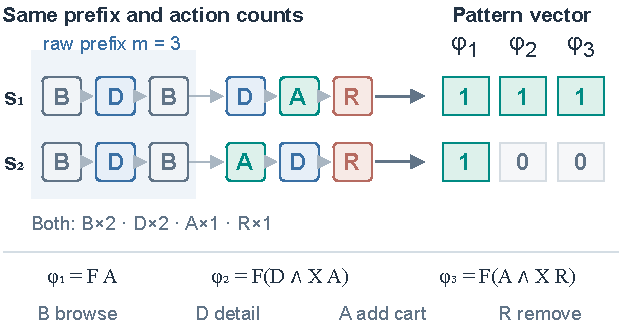
\includegraphics[width=\linewidth]{figures/fig1_patterns.pdf}
\caption{\rev{Why project clickstreams onto patterns? The two toy sessions share their first three events and action counts, yet satisfy different temporal queries. $B,D,A,R$ denote browse, detail, add cart, and remove.}}
\Description{Identical raw prefixes and action counts map to different formula-satisfaction vectors when the later event order changes.}
\label{fig:core-idea}\label{fig:running-example}
\end{figure}
% Introduce the intuition of LTLf
To address this gap, we explore whether temporal logic can provide a compact representation of behavioral patterns in variable-length sessions. Figure~\ref{fig:core-idea} illustrates the core idea of our approach: selected $\mathrm{LTL}_f$ formulas are used as temporal queries to convert full clickstream sessions into compact formula-satisfaction signals for downstream prediction. Specifically, we seek a representation that describes which temporal patterns occur without requiring them to appear at fixed positions.
Linear temporal logic over finite traces ($\mathrm{LTL}_f$) provides a natural language for this purpose. Linear temporal logic (LTL) was originally introduced to specify temporal properties over ordered sequences of states~\cite{pnueli1977temporal}, while $\mathrm{LTL}_f$ evaluates such properties over finite traces with a defined beginning and end~\cite{de2013linear}. This finite characteristic makes it ideally suited to clickstream sessions. Existing approaches often operate directly on the raw event sequence or transform it into learned or handcrafted representations. In contrast, an $\mathrm{LTL}_f$ formula captures high-level patterns across the entire trace. For example, the property that an add-to-cart action occurs somewhere in the session can be expressed as $\mathbf{F}(\mathsf{addCart})$, where $\mathbf{F}$ denotes ``eventually.'' \rev{A more structured pattern, such as a product revisit immediately followed by an add-to-cart action,} can be expressed as $\mathbf{F}(\mathsf{revisit} \wedge \mathbf{X}\mathsf{addCart})$, where $\mathbf{X}$ denotes the next event. Likewise, the condition that browsing continues until a product-detail view occurs can be expressed as $(\mathsf{browse} \;\mathbf{U}\; \mathsf{detail})$, where $\mathbf{U}$ denotes ``until.'' \rev{An eventually formula searches for a witness anywhere in the observed trace, while next and until retain their order and boundary semantics. The resulting fixed-dimensional coordinates retain these explicit temporal meanings.}

% Together, these atomic attributes allow us to map high-level behavioral intuitions into formal $\mathrm{LTL}_f$ specifications.
To evaluate such formulas, a session is represented as a finite symbolic trace $\tau=\langle\sigma_1,\ldots,\sigma_T\rangle$, where each state $\sigma_t$ is a set of attributes describing the event at position $t$. An event may simultaneously satisfy multiple attributes, such as being a product-detail view, having a long dwell time, and representing a revisit to an earlier product. \rev{The complete syntax and finite-trace semantics are presented in Section~\ref{sec:method}.} \rev{Figure~\ref{fig:core-idea} gives an action-level running example. Both sessions begin with $B,D,B$ and contain two browse, two detail, one cart, and one removal event. A first-three raw window and action counts therefore coincide, while the order of later interactions differs. Temporal queries expose this difference in explicitly defined coordinates.}



% Definition of LTLf satisfaction vector z_Phi(tau) and running example.
Formally, given a selected formula basis $\Phi=\{\varphi_1,\ldots,\varphi_K\}$, we represent a session $\tau$ as a $K$-dimensional Boolean satisfaction vector $\mathbf z_\Phi(\tau)=(z_1,\ldots,z_K)\in\{0,1\}^K$, where $z_k=\mathbf1[\tau\models\varphi_k]$. \rev{In Figure~\ref{fig:core-idea}, let $\varphi_1=\mathbf F A$, $\varphi_2=\mathbf F(D\land\mathbf X A)$, and $\varphi_3=\mathbf F(A\land\mathbf X R)$. Session $s_1$ gives $(1,1,1)$, whereas $s_2$ gives $(1,0,0)$. The first-three prefix gives $(0,0,0)$ in both cases.} \rev{The vector dimension $K$ is fixed regardless of session length $T$, yielding a compact and interpretable summary of the available behavior.}

% Data-driven formula mining & Dual-channel synergy (Local raw window + Global LTLf logic)
Rather than manually written rules, candidate formulas are automatically mined from training traces using an $\mathrm{LTL}_f$ formula learner~\cite{wan2024end} \rev{and ranked on a designated development pool. The saved bases used here and their ranking sources are specified in Section~\ref{sec:implementation}.} Overall, this framework provides two complementary prediction channels: the short raw window preserves detailed local event content, while \rev{the formula-satisfaction vector captures selected temporal properties across the available session history.}

% Expected results
\rev{Across three public e-commerce datasets, we examine how this representation changes when the observation boundary is extended, how much it adds beyond counts and adjacent transitions, and which costs move from the neural encoder to feature construction. This connects a compact temporal representation to two concrete uses: summarizing an available session history and predicting a future purchase from a fixed event prefix.}

\paragraph{Contributions}
\begin{itemize}
  \item \rev{\textbf{Logic-guided dual-channel representation.} We combine a short raw sequence with a fixed-dimensional satisfaction vector whose coordinates correspond to explicit temporal behavior properties.}
  \item \rev{\textbf{Trace abstraction and observation scope.} We map observable actions and relational context into event-aligned symbolic traces, and evaluate the same formula basis on a short prefix and the complete available history.}
  \item \rev{\textbf{Matched predictive and computational evaluation.} On three datasets, count and transition controls identify the incremental value of logic at a common observation boundary. Fixed-origin prediction and measured update, memory, and inference costs establish when the compact representation is useful.}
\end{itemize}

\section{Related Work}\label{relatedwork}

This section reviews two main lines of research relevant to our work including clickstream sequence modeling and temporal logic trace representations. We highlight how our approach bridges these domains by transforming full-session $\mathrm{LTL}_f$ verification into a compact predictive vector.

\subsection{Clickstream Sequence Modeling}



\begin{table*}[t]
  \centering
  \small
  \rev{}\caption{Taxonomy of sequential behavior prediction paradigms ($L$: sequence length, $K$: formula basis size / window size, $d$: feature dimension, $|\mathcal{S}|$: state space). \rev{Costs indicate representative encoding operations; retrieval, preprocessing, and implementation details add to these terms.}}
  \label{tab:related_work_taxonomy}
  \begin{tabularx}{\textwidth}{l l c l X}
    \toprule
    \textbf{Paradigm} & \textbf{Context scope} & \textbf{Time complexity} & \textbf{Interpretability} & \textbf{Primary bottleneck} \\
    \midrule
    Probabilistic / Markov~\cite{hatt2020early,ozyurt2022deep} & Short-range & $\mathcal{O}(L \cdot |\mathcal{S}|^2)$ & Explicit (Transitions) & Limited long-range dependence. \\
    RNN / Session embed.~\cite{koehn2020predicting,alves2022will} & Intra-session & $\mathcal{O}(L \cdot d^2)$ & Implicit (Embeddings) & Long-range dependency; opaque states. \\
    Transformers~\cite{black2024trace} & Long-range & $\mathcal{O}(L^2 \cdot d)$ & Heuristic (Attention) & Quadratic attention cost. \\
    Retrieval / Truncation~\cite{li2026lifelong,lin2026mixture} & Subsampled & $\mathcal{O}(K \cdot d)$ or $\mathcal{O}(K^2 \cdot d)$ & Instance-level & Information loss from selected context. \\
    \bottomrule
 
  \end{tabularx}
\end{table*}

Clickstream prediction has been widely studied as a behavioral sequence modeling problem.
Prior work has modeled sequential browsing behavior using recurrent neural networks,
handcrafted representations of browsing trajectories, and other sequence-based predictors
~\cite{koehn2020predicting,requena2020shopper}. To capture dynamic shopping behaviors, probabilistic models such as Markov-modulated point processes (M3PP) detect early user exits~\cite{hatt2020early}, whereas deep Markov models combine latent states with neural components to track shopping phases~\cite{ozyurt2022deep}. Beyond basic sequences, representation learning compresses browsing sessions into dense embeddings for purchase prediction~\cite{alves2022will}. Modern Transformer architectures further extend this paradigm, learning user representations directly from long and feature-rich clickstreams~\cite{black2024trace}. We summarize and compare these main prediction paradigms in Table~\ref{tab:related_work_taxonomy}.



While these approaches confirm the value of temporal signals in clickstreams, processing long, raw behavioral sequences imposes heavy computational overhead. To address this bottleneck, recent long-sequence recommendation methods explore adaptive neural compression and subsequence routing; for instance, Li et al.~\cite{li2026lifelong} apply adaptive subsequence compression for lifelong recommendation, while Lin et al.~\cite{lin2026mixture} propose a theme-aware mixture-of-experts architecture to partition long sequences. Although these methods reduce computational overhead without pure truncation, they rely on dense, implicit latent representations that lack transparency and behavioral interpretability. In this study, we explore whether full-session clickstreams can be efficiently encoded into a compact, human-readable symbolic representation grounded in model-checked $\text{LTL}_f$ formulas.

\rev{Predictive process monitoring makes the observation boundary central by predicting outcomes from incomplete traces. Teinemaa et al.~\cite{teinemaa2019outcome} compare encoding and learning choices across a common benchmark. This motivates our separation of the observed event prefix from the representation constructed on it: aggregate counts and explicit temporal features are compared with the same classifier and the same available events.}

\subsection{Temporal Logic Learning and Trace Representation}

% Introduce temporal logic
While sequence models extract implicit vector embeddings from ordered events, temporal logic provides a formal framework for declarative trace characterization. Through $\text{LTL}_f$~\cite{de2013linear}, behavioral patterns are mapped into explicit logical constraints instead of opaque feature spaces. \rev{Formulas encode temporal properties}, including event occurrences, order dependencies, and conditional invariants across the trace.

Extensive research explores automated learning of temporal specifications from trace examples. Early methods use constraint-solving techniques to learn compact temporal formulae separating positive and negative traces~\cite{neider2018learning,camacho2019learning}. To handle real-world noise and complexity, subsequent work incorporates scalable search and neural temporal-logic learning~\cite{gaglione2022maxsat,valizadeh2024ltl}. Wan et al.~\cite{wan2024end} enable end-to-end $\text{LTL}_f$ formula learning via neural encodings, with recent advances addressing constrained learning and complexity bounds~\cite{wan2024end,10.1109/ICSE55347.2025.00160,bordais2025complexity}. \rev{These studies provide the formula-learning machinery. Our focus is how a frozen learned basis functions as a downstream summary under matched observation and computational conditions.}

Temporal logic has also been applied to trace encoding and log querying in domain-specific workflows. In declarative process mining, the DECLARE framework formulates behavioral constraints using predefined $\text{LTL}_f$ patterns, characterizing event traces by constraint fulfillment and violation~\cite{pesic2007declare}. Di Francescomarino et al.~\cite{di2022making} encode event traces using the satisfaction behavior of declarative temporal patterns, while subsequent work combines declarative and sequential patterns to characterize and explain process outcomes~\cite{di2025business}. \rev{In e-commerce analytics, Hern\'andez et al.~\cite{hernandez2017using} use manually specified LTL formulas for offline log querying.} 

\rev{These lines of work connect temporal specifications, explicit encodings, and prediction.} Our work bridges these paradigms by learning a data-driven $\text{LTL}_f$ formula basis from clickstreams to construct a compact, fixed-dimensional satisfaction vector. \rev{We evaluate this vector jointly with short raw sequences, using counts, dimension-matched adjacent transitions, and fixed-origin prediction to establish its incremental value.}


\section{Logic-Guided Temporal Representation}
\label{sec:method}

This section formalizes the proposed logic-guided temporal representation. Given a clickstream session, we first construct a finite symbolic trace from observable event information. A selected set of LTL$_f$ formulas is then evaluated over the full trace to obtain a fixed-dimensional formula-satisfaction representation, which can be used independently or together with a short raw sequence for downstream prediction.

\rev{Figure~\ref{fig:framework} illustrates how the observed clickstream is projected onto temporal patterns. The raw branch encodes a short window, and the logic branch checks formulas on the available symbolic history.} The resulting formula-satisfaction vector can then be used independently or fused with the raw representation for purchase prediction. The formulation is agnostic to any particular dataset, neural architecture, or formula-learning algorithm. 

\begin{figure*}[t]
\centering
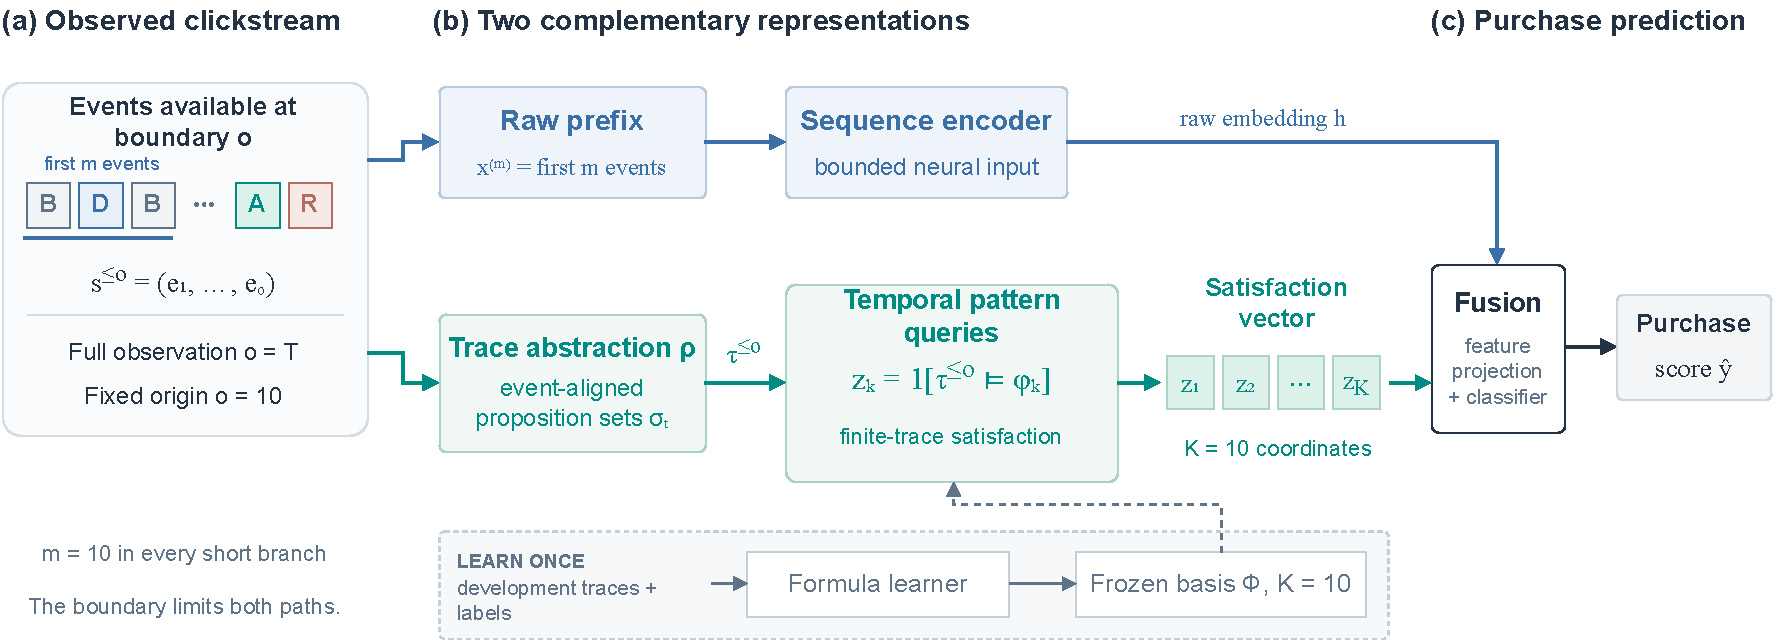
\includegraphics[width=\textwidth]{figures/fig2_framework.pdf}
\caption{\rev{The logic-guided representation separates the raw input budget $m$ from the observation boundary $o$. Both branches use only available events. Event-aligned abstraction and a frozen formula basis produce $K$ explicit pattern coordinates; these complement a bounded raw encoder. Dashed arrows indicate reuse of the basis learned once from development traces.}}
\Description{A bounded raw sequence encoder and a temporal-query encoder share an explicit observation boundary, and feed a fusion predictor. Formula learning is separated from prediction.}
\label{fig:framework}
\end{figure*}


\subsection{Problem Formulation}\label{sec:problem_formulation}
% Define session-level prediction task
Let $\mathcal{D}=\{(s_i,y_i)\}_{i=1}^{N}$ denote a collection of $N$ clickstream sessions, where $s_i$ is a finite session trace and $y_i \in \{0,1\}$ is the session-level prediction target ($y_i=1$ denotes a purchase session and $y_i=0$ otherwise). Each session $s_i=(e_{i,1},e_{i,2},\dots,e_{i,T_i})$ is an event sequence of variable length $T_i$. Each event contains observable information recorded at step $t$, represented in general as $e_{i,t}=(a_{i,t},d_{i,t},p_{i,t},c_{i,t},\dots)$, where $a_{i,t}$ denotes the user action, $d_{i,t}$ denotes timing or dwell-related information, and $p_{i,t}$ and $c_{i,t}$ denote product-level and category-level contexts, respectively.

% Define raw sequence and short window
A conventional sequence predictor operates directly on the complete session $s_i$. To study prediction with reduced raw sequence input, we define $x_i^{(m)}$ as the short observation window consisting of the first $m$ events of session $s_i$:
\begin{equation}
    x_i^{(m)} = (e_{i,1}, e_{i,2}, \dots, e_{i,\min(m, T_i)})
\end{equation}

% Connect to Running Example in Introduction
\rev{As illustrated in Figure~\ref{fig:core-idea}, the raw channel preserves the first $m$ events, while formula satisfaction can retain properties witnessed beyond that window. The framework keeps the available history explicit so that these two channels can also be compared at a common observation boundary.}

% Formula-satisfaction channel & general prediction interface
Our goal is to learn a predictive mapping $f: (x_i^{(m)}, s_i) \to \hat{y}_i$ that mitigates the information loss of the truncated window $x_i^{(m)}$ by incorporating global logic-derived behavioral properties evaluated over the full sequence $s_i$. The following subsections formalize the abstraction mechanism, logic semantics, formula learning, and the unified prediction interfaces.




\rev{We distinguish the raw input budget $m$ from the observation boundary $o_i$. Write $s_i^{\leq o_i}=(e_{i,1},\ldots,e_{i,o_i})$ for the events available to a predictor. Full-observation evaluation uses $o_i=T_i$, whereas fixed-origin prediction uses $o_i=10$ for both branches. In the latter setting, $s_i$ in the following definitions means this observed prefix, and the target is purchase within a specified future event horizon. Formula satisfaction is always evaluated on the supplied finite trace.}

\subsection{Trace Abstraction over Atomic Propositions}
\label{sec:trace_abstraction}

% 1. Direct cut-in from formal requirements (Formal yet concise)
$\text{LTL}_f$ formulas require input sequences composed of Boolean atomic propositions. However, raw clickstream logs contain heterogeneous signals, including continuous dwell times, categorical actions, and relational contexts. Trace abstraction converts these raw event sequences into symbolic traces suitable for temporal logic evaluation. We use an abstraction scheme $r$ to specify which raw signals are encoded into the proposition vocabulary $\mathcal{P}^{(r)}$.

% 2. Formal abstraction function (e_{i,t} -> \sigma_{i,t} -> \tau_i)
Formally, let $h_{i,t} = (e_{i,1},\dots,e_{i,t})$ denote the prefix history of session $s_i$ up to step $t$. An abstraction function $\rho^{(r)}$ maps each raw event $e_{i,t}$ and its contextual prefix $h_{i,t}$ to a state $\sigma_{i,t}^{(r)}$ consisting of satisfied atomic propositions:
\begin{equation}
    \sigma_{i,t}^{(r)} = \rho^{(r)}(e_{i,t}, h_{i,t}) \subseteq \mathcal{P}^{(r)}
\end{equation}
Sequentially evaluating $\rho^{(r)}$ across all $T_i$ steps yields the full-session symbolic trace:
\begin{equation}
    \tau_i^{(r)} = (\sigma_{i,1}^{(r)}, \sigma_{i,2}^{(r)}, \dots, \sigma_{i,T_i}^{(r)})
\end{equation}

% 3. Conceptual Contribution: Simultaneous Multi-Property Representation
By construction, since each state is defined as a subset of propositions ($\sigma_{i,t}^{(r)} \in 2^{\mathcal{P}^{(r)}}$), a single temporal position $t$ can simultaneously satisfy multiple heterogeneous properties, such as an action predicate, a dwell-time condition, and a history-dependent product relation. This multi-property formulation allows our framework to incorporate richer feature modalities simply by expanding the vocabulary $\mathcal{P}^{(r)}$, leaving the downstream $\text{LTL}_f$ evaluation mechanism completely invariant.

\rev{For example, a detail event on product $p_1$ with a long dwell can map to $\{D,\mathsf{longDwell},\mathsf{fp}\}$ on its first occurrence. A later event on the same product activates $\mathsf{rp}$. The action and relation propositions used in the experiments describe product availability, first occurrence/revisit, repetition, distinct-product counts, and product/category changes. They depend only on the current event and its prefix history.}


\subsection{\texorpdfstring{LTL\textsubscript{f}}{LTLf} over Symbolic Traces}
\label{sec:ltlf_semantics}

Given a proposition vocabulary $\mathcal{P}^{(r)}$ induced by an abstraction scheme $r$, Linear Temporal Logic over Finite Traces ($\text{LTL}_f$)~\cite{baier2006planning,de2013linear,wan2024end} expresses temporal constraints over symbolic clickstream sequences. Formulas are constructed from atomic propositions using standard Boolean connectives and temporal operators, governed by the grammar:
\begin{equation}
    \varphi ::= p \mid \neg\varphi \mid \varphi_1 \land \varphi_2 \mid \mathbf{X}\varphi \mid \varphi_1 \mathbf{U} \varphi_2,
\end{equation}
where $p \in \mathcal{P}^{(r)}$, $\mathbf{X}$ denotes the \emph{next} operator, and $\mathbf{U}$ denotes the \emph{until} operator. As standard shorthands, we define \emph{eventually} as $\mathbf{F}\varphi \equiv \top \mathbf{U} \varphi$ and \emph{globally} as $\mathbf{G}\varphi \equiv \neg\mathbf{F}\neg\varphi$.

We interpret $\text{LTL}_f$ formulas under finite-trace semantics. For a finite trace $\tau_i^{(r)} = (\sigma_{i,1}^{(r)}, \dots, \sigma_{i,T_i}^{(r)})$, let $\tau_i^{(r)}, t \models \varphi$ denote that $\varphi$ holds at position $t \in \{1, \dots, T_i\}$. The semantics is given by:
(i)~$\tau_i^{(r)}, t \models p \iff p \in \sigma_{i,t}^{(r)}$;
(ii)~$\tau_i^{(r)}, t \models \mathbf{X}\varphi \iff t < T_i \land \tau_i^{(r)}, t+1 \models \varphi$; and
(iii)~$\tau_i^{(r)}, t \models \varphi_1 \mathbf{U} \varphi_2 \iff \exists j \in [t, T_i]$ s.t.\ $\tau_i^{(r)}, j \models \varphi_2$ and $\forall k \in [t, j-1], \tau_i^{(r)}, k \models \varphi_1$.
Finally, a trace satisfies $\varphi$, written $\tau_i^{(r)} \models \varphi$, if $\tau_i^{(r)}, 1 \models \varphi$.

\rev{This formulation evaluates properties such as $\mathbf{F}(\mathsf{A})$ and $\mathbf{F}(\mathsf{rp}\land\mathbf{X}\mathsf{A})$ over the supplied sequence. On a prefix, false means that the property is false on that finite prefix; extending the trace can change its truth value.}



\subsection{Temporal Formula Learning and Selection}
\label{sec:formula_learning}

In this study, we obtain temporal formulas automatically from labeled traces rather than manually specifying the representation basis. For a given abstraction scheme $r$, let $\mathcal{T}_{\text{tr}}^{(r)} = \{(\tau_i^{(r)}, y_i)\}_{i=1}^{N_{\text{tr}}}$ denote the set of symbolic training traces. Following the temporal formula learning protocol in~\cite{wan2024end}, a formula learner $\mathcal{FL}$ extracts candidate temporal logic patterns, \rev{such as $\mathbf{F}(\mathsf{A})$ or $\mathbf{F}(\mathsf{D}\land\mathbf{X}\mathsf{A})$ in Figure~\ref{fig:core-idea}} from $\mathcal{T}_{\text{tr}}^{(r)}$, yielding a candidate collection:
\begin{equation}
    \mathcal{C}^{(r)} = \mathcal{FL}\left(\mathcal{T}_{\text{tr}}^{(r)}\right)
\end{equation}

\rev{Candidate formulas are evaluated and ranked by their class-separating performance on a designated development pool. This pool can be held-out validation data or the formula-fitting training pool, as documented for each saved basis in Section~\ref{sec:implementation}. Selecting the top-$K$ formulas defines the temporal formula basis:}
\begin{equation}
    \Phi^{(r)} = \left\{\varphi_1^{(r)}, \varphi_2^{(r)}, \dots, \varphi_K^{(r)}\right\} \subset \mathcal{C}^{(r)}
\end{equation}

Once the formula basis $\Phi^{(r)}$ is determined, it is completely frozen for all subsequent downstream training and evaluation. For any given trace $\tau_i^{(r)}$ across training, validation, or test splits, the model checker evaluates each formula in $\Phi^{(r)}$ against $\tau_i^{(r)}$ to construct the final formula-satisfaction representation, as formalized next.


\subsection{Formula-Satisfaction Representation}\label{formula_satisfaction_repre}

Given the fixed temporal formula basis $\Phi^{(r)} = \{\varphi_1^{(r)}, \dots, \varphi_K^{(r)}\}$, we map each variable-length symbolic trace $\tau_i^{(r)}$ into a canonical $K$-dimensional binary vector $z_i^{(r)} \in \{0, 1\}^K$. Formally, the mapping $V_{\Phi^{(r)}}$ is defined coordinate-wise as:
\begin{equation}
    z_i^{(r)} = V_{\Phi^{(r)}}\left(\tau_i^{(r)}\right) = \left[ \mathbb{I}\left[\tau_i^{(r)} \models \varphi_1^{(r)}\right], \dots, \mathbb{I}\left[\tau_i^{(r)} \models \varphi_K^{(r)}\right] \right]^\top,
\end{equation}
where $\mathbb{I}[\cdot]$ denotes the indicator function, and $\models$ represents the $\text{LTL}_f$ satisfaction relation over the complete trace $\tau_i^{(r)}$.

This representation complements the local observation window $x_i^{(m)}$ in two key respects. First, while $x_i^{(m)}$ preserves detailed local event dynamics, $z_i^{(r)}$ provides global behavioral coverage by evaluating logic properties over the full session. Second, because the basis dimension $K$ is fixed, $z_i^{(r)}$ maps arbitrary-length sessions into a shared $K$-dimensional feature space, activating identical coordinates whenever the underlying temporal patterns are satisfied regardless of session length or event positions.



\subsection{Prediction Interfaces}
\label{sec:prediction_interfaces}

\rev{The raw, satisfaction-only, and fusion interfaces use the following inputs:
\begin{align}
\hat y_i^{\rm raw}&=f_{\theta_{\rm raw}}(x_i^{(m)}), &
\hat y_i^{\rm sat}&=f_{\theta_{\rm sat}}(z_i^{(r)}),\notag\\
\hat y_i^{\rm fus}&=f_{\theta_{\rm fus}}(x_i^{(m)},z_i^{(r)}).
\end{align}
The experiments evaluate raw and fusion prediction. Fusion encodes the short raw sequence and the symbolic vector in separate branches, then combines them before classification (Figure~\ref{fig:framework}). This retains local event content together with selected temporal properties of the available history.}

\subsection{Properties and Computational Cost}
\label{sec:properties_cost}

By construction, the formula-satisfaction vector $z_i^{(r)}$ exhibits three desirable properties: (i)~\textbf{Fixed Dimensionality:} A formula basis $\Phi^{(r)}$ of size $K$ maps arbitrary-length sessions into a uniform $\{0,1\}^K$ space, bypassing the need for sequence padding or truncation. (ii)~\textbf{Deterministic Inference:} Once $r$ and $\Phi^{(r)}$ are fixed, $V_{\Phi^{(r)}}(\tau_i^{(r)})$ provides a label-free, deterministic encoding for any unseen session. (iii)~\textbf{Explicit Semantics:} Each coordinate encodes the truth value of a distinct $\mathrm{LTL}_f$ rule, offering transparent temporal properties instead of opaque latent representations.

\rev{Let $L$ be the available trace length and $\overline{|\varphi|}$ the mean formula size. With a fixed basis, finite-trace checking costs $\mathcal O(L|\varphi_k|)$ per formula, giving
\begin{align}
C_{\rm MC}(L)&=\mathcal O\!\left(L\sum_{k=1}^K|\varphi_k|\right)
=\mathcal O(KL\overline{|\varphi|}),\label{eq:model_checking_cost}\\
C_{\rm fusion}&=C_{\rm raw}(m)+\mathcal O(KL\overline{|\varphi|}).\label{eq:dual_channel_cost}
\end{align}
Thus, the neural branch is bounded by $m$, while model checking scales linearly in $L$ for a fixed basis. For a Transformer of hidden width $d$, the comparison becomes
\begin{align}
C_{\rm full}^{\rm Tr}&=\mathcal O(L^2d+Ld^2),\notag\\
C_{\rm fusion}^{\rm Tr}&=\mathcal O(m^2d+md^2+KL\overline{|\varphi|}).\label{eq:transformer_dual_cost}
\end{align}
The quadratic attention term is restricted to the raw window. The $K$ coordinates retain exactly the properties expressed by the basis, while the raw branch preserves detailed content in its prefix. This decomposition motivates measuring neural updates, summary construction, and feature-inclusive inference separately. Formula learning and event abstraction are setup steps outside this per-session checking-and-encoding analysis.}

\begin{revblock}
\section{Empirical Study}
\label{sec:empirical}
The empirical study connects observation scope, representation content, and computational cost. We begin with the predictive performance of full-history and short-input representations, then examine the information contributed by counts, adjacent transitions, and temporal logic. Fixed-origin purchase prediction places these summaries at a common observation boundary. Measurements of neural updates, feature construction, and GPU allocation complete the analysis of their predictive and computational tradeoffs.

\subsection{Experimental Protocol}
\label{sec:settings}\label{sec:implementation}
We evaluate Coveo~\cite{CoveoSIGIR2021}, Electronics\footnote{\rev{\url{https://www.kaggle.com/datasets/mkechinov/ecommerce-purchase-history-from-electronics-store}}}, and Cosmetics\footnote{\rev{\url{https://www.kaggle.com/datasets/mkechinov/ecommerce-events-history-in-cosmetics-shop}}}. The raw input is action and product/category IDs; the symbolic vocabulary is Act+Rel. We fix the raw window at the first $m=10$ events and reuse $K=10$ formulas per dataset. This keeps the information fields and representation size fixed across the scope and summary comparisons.

\begin{table*}[t]
\centering\small\setlength{\tabcolsep}{4pt}
\caption{\rev{Evaluation cohorts, split seed 42. $\pi_{\rm full}$ and $\pi_{10}$ are test positive percentages for full observation and next-ten-event prediction, respectively. The three future horizons share the same event-10 cohort.}}
\label{tab:cohorts}
\begin{revblock}
\begin{tabular}{@{}lrrrc@{}}
\toprule
Dataset & Full observation: train / val. / test & At event 10: train / val. / test & $\pi_{\rm full}$ / $\pi_{10}$ & Raw cap \\
\midrule
Coveo & 179,616 / 38,489 / 38,490 & 56,853 / 12,353 / 12,202 & 20.0 / 17.3 & 200 \\
Electronics & 73,717 / 10,531 / 21,062 & 2,407 / 339 / 759 & 20.0 / 20.7 & 512 \\
Cosmetics & 91,477 / 12,804 / 25,836 & 14,565 / 2,089 / 4,185 & 19.9 / 28.8 & 200 \\
\bottomrule
\end{tabular}
\end{revblock}

\end{table*}

\paragraph{Observation and targets.}
In \emph{full observation}, positive histories stop immediately before first purchase and negative histories retain all recorded events. The target is whether the original session purchases. This evaluates complete available-history representations at a purchase-relative cutoff. In \emph{fixed-origin prediction}, sessions must reach ten events before any purchase; every feature uses events 1--10, and the target is first purchase in the next $H\in\{5,10,20\}$ recognized events. The purchase event counts toward $H$; a later purchase or a session ending without purchase within the horizon receives label zero. Table~\ref{tab:cohorts} gives both populations. The historical sampling produces approximately 20\% positive full-observation sessions. Cosmetics preserves its split assignments and removes empty purchase-cutoff histories, including 34 positive test sessions.

\paragraph{Formula provenance and splits.}
Coveo and Cosmetics use the first ten formulas of saved ranked 20-formula bases; Electronics uses its saved ten-formula basis. Fitting and ranking used training traces for Coveo and Electronics, and training and validation traces, respectively, for Cosmetics. The protected Coveo split contains all 20,000 formula-fitting traces in downstream training. Cosmetics transfers its basis learned from historical purchase-masked traces to the purchase-cutoff task; 526 fitting and 259 ranking histories in that source extended beyond first purchase. Test sessions remain outside these pools. Cosmetics is user-disjoint; Electronics evaluates unseen sessions but shares 2,784 users between training and test. Coveo user IDs are unavailable. Each dataset retains one split and one frozen basis throughout the study.

\paragraph{Predictors and controls.}
Five separately fitted neural conditions use the dataset-specific Transformer implementations: Full raw, Short raw, Short + Prefix-LTLf, Short + Counts, and Short + Full-LTLf. Prefix-LTLf checks only the first ten events; Counts and Full-LTLf use the entire available symbolic history. Counts contains proposition frequencies and length, scaled with training data. Full raw uses the caps in Table~\ref{tab:cohorts}: these truncate zero, one, and 21 test histories in Coveo, Electronics, and Cosmetics. Symbolic summaries retain all available events. Coveo trains for 25 epochs (batch 256), selects by validation F1 at threshold 0.5, and then chooses a validation-F1 threshold. Electronics uses at most 20 epochs, patience 4, batch 256, validation AP selection, and threshold 0.5. Cosmetics uses at most 25 epochs, patience 5, train/evaluation batches 512/1,024, validation MCC selection, and threshold 0.5.

For a shared-classifier comparison, we fit L2-regularized logistic regression ($C=1$) to position-wise one-hot raw-prefix tokens and standardized summary features. A fixed validation grid selects the MCC threshold. Logic and transitions each contribute ten Boolean features. A transition indicates whether a proposition pair occurs in adjacent states; candidates present and absent in at least 20 training sessions are ranked by the absolute purchase/non-purchase prevalence difference. Full-history and prefix transitions are selected separately. The prefix transition basis and the formula basis are fixed across $H$, using the original session-purchase target for their selection.

\paragraph{Metrics and uncertainty.}
We report MCC and average precision (AP). Predictive entries are \emph{estimate $\pm$ one bootstrap standard error} (SE), computed from 1,500 resamples with models and thresholds fixed. Users are resampled in Electronics and Cosmetics, sessions in Coveo; paired differences use the same resample for both models. SE is the sample standard deviation of bootstrap estimates, without division by $\sqrt{1{,}500}$; the displayed $\pm$ is not a 95\% confidence interval. This describes conditional test-sampling uncertainty. Separately, training seeds 42/43/44 measure optimization variation for Counts and Full-LTLf on the same split, reported as mean $\pm$ sample SD. Runtime repeats also use mean $\pm$ sample SD, with their own measurement boundary.

\subsection{Observation Scope and Prediction}
\label{sec:scope}
The full-observation comparison separates the raw sequence budget from the history available to each summary (Table~\ref{tab:neural}). On Coveo, Full-LTLf raises MCC from 0.653 for Short raw to 0.865, close to Full raw at 0.868. Counts reaches 0.867 and retains the AP of Full raw. Electronics shows a smaller aggregate change, while Cosmetics benefits most from Counts. These differences across datasets motivate examining both summary coverage and feature content.

\begin{table*}[t]
\centering\small\setlength{\tabcolsep}{4pt}
\caption{\rev{Neural prediction on full-observation histories. Each short raw branch uses the first ten events. Prefix-LTLf sees those events; Counts and Full-LTLf see the full available history. Entries are seed-42 estimate $\pm$ bootstrap SE; bold marks the largest point estimate per column.}}
\label{tab:neural}
\begin{revblock}
\begin{tabular}{@{}lrrrrrr@{}}
\toprule
& \multicolumn{2}{c}{Coveo} & \multicolumn{2}{c}{Electronics} & \multicolumn{2}{c}{Cosmetics} \\
\cmidrule(lr){2-3}\cmidrule(lr){4-5}\cmidrule(lr){6-7}
Input & MCC & AP & MCC & AP & MCC & AP \\
\midrule
Full raw & \bse{0.868}{0.003} & \vse{0.904}{0.004} & \bse{0.711}{0.005} & \bse{0.734}{0.008} & \vse{0.562}{0.006} & \vse{0.608}{0.008} \\
Short raw & \vse{0.653}{0.005} & \vse{0.797}{0.005} & \vse{0.693}{0.005} & \vse{0.723}{0.008} & \vse{0.567}{0.006} & \vse{0.594}{0.008} \\
Short + Prefix-LTLf & \vse{0.654}{0.005} & \vse{0.800}{0.005} & \vse{0.687}{0.005} & \vse{0.717}{0.008} & \vse{0.610}{0.005} & \vse{0.644}{0.008} \\
Short + Counts & \vse{0.867}{0.003} & \bse{0.905}{0.004} & \vse{0.696}{0.005} & \vse{0.721}{0.008} & \bse{0.648}{0.005} & \bse{0.717}{0.008} \\
Short + Full-LTLf & \vse{0.865}{0.003} & \vse{0.878}{0.004} & \vse{0.702}{0.005} & \vse{0.722}{0.008} & \vse{0.621}{0.005} & \vse{0.658}{0.008} \\
\bottomrule
\end{tabular}
\end{revblock}

\end{table*}

\begin{figure}[t]
\centering
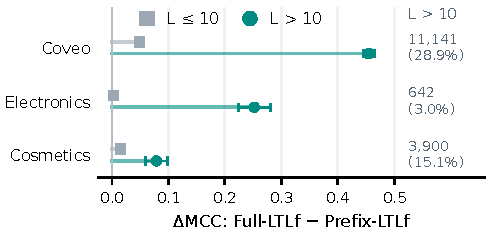
\includegraphics[width=\linewidth]{figures/rq1_scope.pdf}
\caption{\rev{Observation-scope gains are concentrated in histories extending beyond the raw window. Paired Full-LTLf minus Prefix-LTLf MCC, split by length; bars show one bootstrap SE. Right labels give long-history counts and shares.}}
\Description{Scope gains on short and long histories, with long-history population sizes.}
\label{fig:scope}
\end{figure}

The scope effect is concentrated in histories with $L>10$ (Figure~\ref{fig:scope}): the paired MCC gains are $0.455\pm0.009$, $0.252\pm0.029$, and $0.079\pm0.019$ for Coveo, Electronics, and Cosmetics. Only 3.0\% of Electronics test histories exceed ten events, explaining why its aggregate change is modest. For $L\leq10$, both vectors agree for a given history; fitted predictors can still differ because each condition is trained separately. The learned Electronics formula $\mathbf{X}(\top\,\mathbf{U}\,a)$ illustrates the mechanism: an add-to-cart at event 11 can change a false prefix coordinate to true on the longer trace. Extending scope exposes additional evidence through an explicit temporal query.

\subsection{Counts, Transitions, and Logic}
\label{sec:controls}
At a matched observation scope, counts, transitions, and logic encode different aspects of behavior. Counts retain activity intensity, while relation atoms summarize history through revisits and product changes. Action counts sum to length. In the linear controls, adding length raises Coveo MCC from 0.638 to 0.715; action counts reach 0.844. Cosmetics reaches 0.600 with Act+Rel counts versus 0.592 with action counts. These controls identify strong non-sequential information before testing temporal order.

\begin{table*}[t]
\centering\small\setlength{\tabcolsep}{4pt}
\caption{\rev{Count and temporal summaries with matched linear predictors, estimate $\pm$ bootstrap SE. Every row includes the raw prefix. LTLf and Transitions each add ten Boolean coordinates; Both adds both sets. Counts includes length in (a); all histories have length ten in (b). Bold marks the largest point estimate within each panel.}}
\label{tab:linear}
\begin{revblock}
\begin{tabular}{@{}lrrrrrr@{}}
\toprule
& \multicolumn{2}{c}{Coveo} & \multicolumn{2}{c}{Electronics} & \multicolumn{2}{c}{Cosmetics} \\
\cmidrule(lr){2-3}\cmidrule(lr){4-5}\cmidrule(lr){6-7}
Input & MCC & AP & MCC & AP & MCC & AP \\
\midrule
\multicolumn{7}{@{}l}{\textit{(a) Full-observation summaries}} \\
Raw prefix & \vse{0.638}{0.005} & \vse{0.771}{0.005} & \vse{0.655}{0.005} & \vse{0.635}{0.009} & \vse{0.589}{0.006} & \vse{0.629}{0.008} \\
+ Counts & \vse{0.843}{0.003} & \vse{0.869}{0.004} & \vse{0.657}{0.005} & \vse{0.639}{0.009} & \vse{0.599}{0.006} & \vse{0.656}{0.008} \\
+ Counts + LTLf & \vse{0.860}{0.003} & \vse{0.889}{0.004} & \vse{0.687}{0.005} & \vse{0.666}{0.008} & \bse{0.627}{0.006} & \vse{0.670}{0.008} \\
+ Counts + Transitions & \vse{0.863}{0.003} & \vse{0.889}{0.004} & \vse{0.691}{0.005} & \vse{0.678}{0.008} & \vse{0.623}{0.006} & \vse{0.668}{0.008} \\
+ Counts + Both & \bse{0.866}{0.003} & \bse{0.893}{0.004} & \bse{0.694}{0.005} & \bse{0.679}{0.008} & \vse{0.625}{0.006} & \bse{0.671}{0.008} \\
\midrule
\multicolumn{7}{@{}l}{\textit{(b) Event-10 prediction, next 10 events}} \\
Raw prefix & \vse{0.446}{0.009} & \vse{0.448}{0.011} & \vse{0.208}{0.034} & \vse{0.343}{0.035} & \vse{0.109}{0.016} & \vse{0.365}{0.013} \\
+ Counts & \vse{0.447}{0.010} & \vse{0.457}{0.011} & \vse{0.217}{0.035} & \vse{0.363}{0.036} & \vse{0.166}{0.015} & \vse{0.405}{0.014} \\
+ Counts + LTLf & \bse{0.475}{0.010} & \vse{0.478}{0.011} & \bse{0.289}{0.036} & \bse{0.393}{0.039} & \vse{0.188}{0.015} & \vse{0.417}{0.014} \\
+ Counts + Transitions & \vse{0.467}{0.010} & \vse{0.474}{0.011} & \vse{0.269}{0.031} & \vse{0.390}{0.038} & \bse{0.189}{0.015} & \vse{0.421}{0.014} \\
+ Counts + Both & \vse{0.471}{0.010} & \bse{0.480}{0.011} & \vse{0.266}{0.032} & \vse{0.389}{0.038} & \vse{0.185}{0.015} & \bse{0.422}{0.014} \\
\bottomrule
\end{tabular}
\end{revblock}

\end{table*}

With Counts retained, LTLf increases full-observation MCC by $0.017\pm0.002$, $0.030\pm0.003$, and $0.027\pm0.004$ (Table~\ref{tab:linear}a). Ten selected adjacent transitions give gains of 0.020, 0.034, and 0.024. Both summaries therefore capture useful information beyond the count scale, with similar point estimates. The direct LTLf-minus-Transitions MCC differences are $-0.003\pm0.002$, $-0.004\pm0.002$, and $0.003\pm0.003$.

Replacing Counts with Full-LTLf in a neural branch is a different comparison from adding logic to Counts in a linear model. Across training seeds 42/43/44, the paired neural MCC differences average $-0.0011\pm0.0009$, $-0.0108\pm0.0172$, and $-0.0259\pm0.0018$ (mean $\pm$ SD). Counts is consistently ahead on Coveo and Cosmetics; Electronics changes ordering across seeds. Together, the experiments establish counts as an essential baseline and logic as a useful, explicitly interpretable addition in the shared linear classifier.

\subsection{Fixed-Origin Purchase Prediction}
\label{sec:fixed}
Fixed-origin prediction places all representations at the same event-10 boundary and targets purchase in events 11--20 (Table~\ref{tab:linear}b). Every input branch uses only events 1--10. Adding LTLf to Counts raises MCC by $0.028\pm0.006$, $0.072\pm0.026$, and $0.022\pm0.009$. The direct differences from adjacent transitions are $0.007\pm0.004$, $0.020\pm0.025$, and $-0.001\pm0.008$. Logic retains incremental value at the common observation boundary, while simple ordered features remain competitive.

\begin{figure*}[t]
\centering
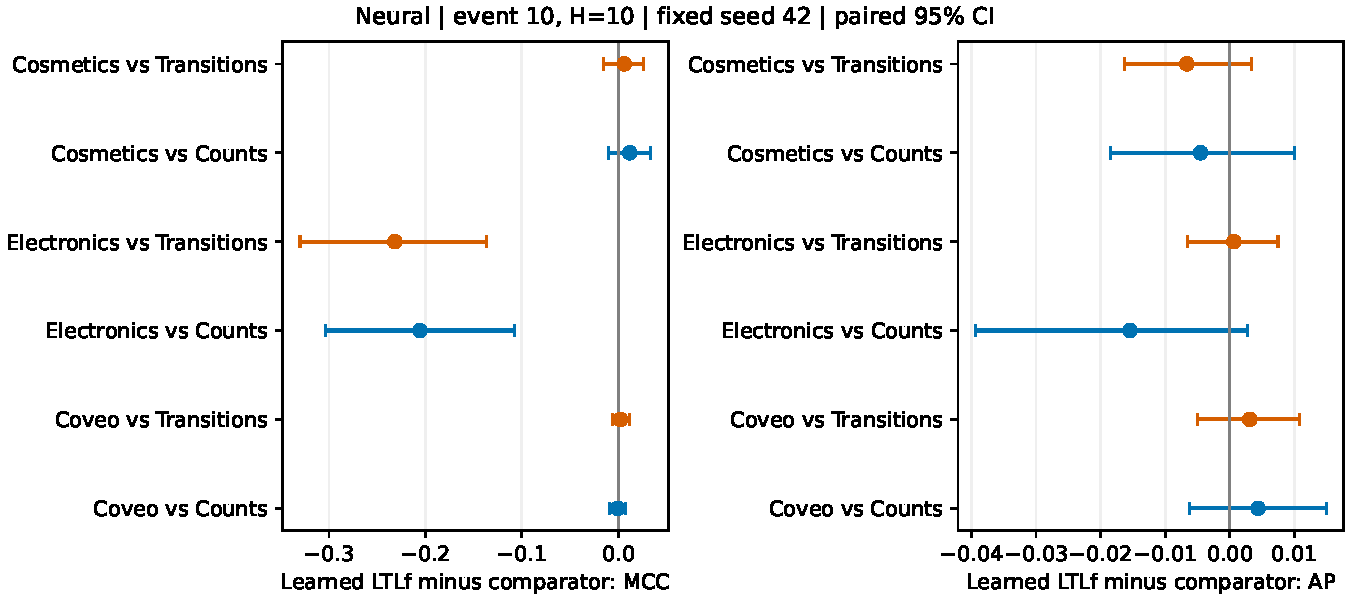
\includegraphics[width=\textwidth]{figures/fixed_neural_differences.pdf}
\caption{\rev{Incremental neural value of LTLf at event 10 with $H=10$. Points use the prespecified seed-42 models and validation-selected thresholds; bars are paired percentile 95\% confidence intervals from 1,500 resamples. Coveo resamples sessions; Electronics and Cosmetics resample users. These conditional intervals are distinct from the training-seed SD in Table~\ref{tab:fixed-neural-new}.}}
\Description{Paired MCC and AP differences from Counts and Transitions, including negative Electronics MCC differences.}
\label{fig:fixed-neural-new}
\end{figure*}

The horizon analysis considers purchases within the next 5, 10, or 20 events (retained in the supplementary horizon results). The LTLf and transition point estimates improve over Counts at all three horizons in all three datasets; combining them gives no uniform further gain. Test purchase prevalence at $H=5/10/20$ is 9.4/17.3/28.1\% for Coveo, 15.5/20.7/24.2\% for Electronics, and 16.9/28.8/43.1\% for Cosmetics. AP comparisons consequently refer to models within the same horizon. This fixed-origin experiment connects the representation to a future event outcome, using the same available information for every summary.

\subsection{Matched Neural and Template Controls}
\begin{table}[t]
\centering\small\setlength{\tabcolsep}{3pt}
\caption{\rev{Fixed-origin neural prediction, event 10 and $H=10$. All rows include the same first-ten-event raw encoder within each dataset. Values are mean $\pm$ sample SD over training seeds 42, 43, and 44.}}
\label{tab:fixed-neural-new}
\resizebox{\columnwidth}{!}{\begin{tabular}{llcc}
\toprule Dataset & Input & MCC & AP \\
\midrule
Coveo & Raw & $0.469\pm0.003$ & $0.513\pm0.006$ \\
 & + Counts & $0.479\pm0.006$ & $0.516\pm0.003$ \\
 & + Counts + Transitions & $0.480\pm0.004$ & $0.512\pm0.003$ \\
 & + Counts + LTLf & $0.479\pm0.002$ & $0.518\pm0.004$ \\
\midrule
Electronics & Raw & $0.251\pm0.029$ & $0.371\pm0.023$ \\
 & + Counts & $0.233\pm0.035$ & $0.378\pm0.016$ \\
 & + Counts + Transitions & $0.286\pm0.007$ & $0.360\pm0.026$ \\
 & + Counts + LTLf & $0.187\pm0.128$ & $0.359\pm0.021$ \\
\midrule
Cosmetics & Raw & $0.036\pm0.021$ & $0.315\pm0.009$ \\
 & + Counts & $0.232\pm0.008$ & $0.436\pm0.004$ \\
 & + Counts + Transitions & $0.237\pm0.008$ & $0.438\pm0.004$ \\
 & + Counts + LTLf & $0.231\pm0.017$ & $0.431\pm0.003$ \\
\bottomrule
\end{tabular}}
\end{table}
The new comparison holds the observation boundary, raw encoder, 64-wide classification head, 25-epoch cap, patience 5, batch size 256, and optimizer settings fixed across four conditions. Vocabularies and scalers use training prefixes only. Validation AP selects checkpoints, followed by a validation-MCC threshold grid. These rules define the new controlled comparison and differ from some historical full-observation settings. The split and frozen formula bases remain unchanged; each summary uses only events 1--10.

Table~\ref{tab:fixed-neural-new} does not show a stable incremental benefit from LTLf over Counts. The mean MCC differences are $-0.0003$, $-0.0453$, and $-0.0005$ for Coveo, Electronics, and Cosmetics. Electronics has substantial initialization variation: LTLf MCC is $0.187\pm0.128$. Its prespecified seed-42 MCC difference from Counts is $-0.206$ (paired 95\% CI $[-0.304,-0.108]$), whereas its AP difference is $-0.015$ ($[-0.039,0.003]$). Figure~\ref{fig:fixed-neural-new} reports all primary paired contrasts. This fixed-model result is not a statement about the mean across initializations, and intervals crossing zero are not evidence of equivalence.

Under the Table~\ref{tab:linear} logistic setup, ten selected Boolean DECLARE-style coordinates yield MCC $0.470$, $0.266$, and $0.201$, compared with frozen learned LTLf $0.475$, $0.289$, and $0.188$. Existence, response, strict precedence, and chain-response candidates use the same proposition vocabulary. Template and re-ranked controls share training ranking IDs, eventual-purchase labels, an absolute-support-gap objective, and empirical-column deduplication. The frozen basis retains its historical selection protocol, so candidate generation is not fully matched. All learned-versus-template MCC and AP intervals cross zero; these experiments do not establish added value from automatic learning. The Electronics pool has only four usable distinct columns after the common prefix filter, precluding its optional ten-feature re-ranking sensitivity arm.

\begin{table}[t]
\centering\footnotesize
\caption{\rev{Representative actual frozen formulas; $a$ is add-to-cart. Full original syntax, provenance, and train/validation satisfaction rates appear in the experiment supplement.}}
\label{tab:actual-formulas}
\begin{tabular}{lll}\toprule Dataset/index & Finite-trace form & Interpretation \\
\midrule
Coveo/3 & $\mathbf{F}\mathbf{X}^{2}a$ & Cart at event 3 or later \\
Electronics/1 & $\mathbf{X}\mathbf{F}a$ & Cart after event 1 \\
Cosmetics/1 & $hp\,\mathbf{U}\,a$ & Product-present until cart \\
Cosmetics/6 & $\mathbf{X}hp$ & Product at event 2 \\
\bottomrule\end{tabular}
\end{table}
Exact finite-trace checking distinguishes all pairs within each ten-formula basis, yet observed columns can coincide. Cosmetics $\mathbf{X}hp$ is constant in the event-10 train/validation cohort, and $hp\,\mathbf{U}\,a$ coincides there with cart occurrence. Such empirical identities are not logical equivalences over arbitrary multi-proposition traces. These formulas support explicit occurrence and guarded temporal summaries, not a claim that complex long-range dependencies were learned.

Prior DECLARE encoding~\cite{di2022making} separates violations from satisfaction and can distinguish vacuous cases, and combines Fisher-score ranking with a coverage rule. Our small baseline instead merges both forms of satisfaction into one Boolean value and selects ten columns by the declared support-gap rule. The experimental distinction is therefore the candidate basis and its integration with a short raw encoder, not the invention of logic-based trace encoding.

A separate Cosmetics source control relearns formulas from pre-purchase histories while retaining eventual-purchase targets and the recovered learner settings. The frozen and relearned bases yield MCC 0.1875 and 0.1890, and AP 0.4172 and 0.4142. The user-cluster paired differences are $+0.0015$ (95\% CI $[-0.0096,0.0132]$) for MCC and $-0.0030$ ($[-0.0063,0.0005]$) for AP. Neither establishes a source benefit. Empty pre-purchase traces exclude 45 fitting and 21 ranking sessions without replacement; CPU execution also differs from the historical GPU run. This is a separate refit, not a replacement selected by test scores. Details and the full basis-source table appear in the supplement.

\subsection{Computational Cost and Efficiency}
\label{sec:compute}
\begin{figure*}[t]
\centering
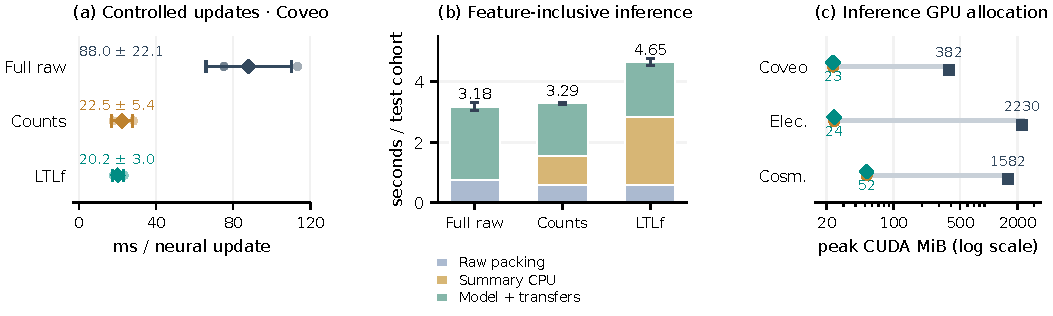
\includegraphics[width=\textwidth]{figures/rq4_cost.pdf}
\caption{\rev{Computational profile of full raw and short-input fusion. (a) Coveo neural-update mean $\pm$ SD, with all three repetition means shown as small dots. (b) Coveo test-cohort inference decomposed into raw packing, symbolic summary construction, and model/transfers; bars on totals show SD. (c) Peak inference CUDA allocation across datasets. Colors in (a,c) identify Full raw, Counts, and LTLf; the two short summaries have nearly identical allocation.}}
\Description{Controlled update costs, decomposed inference costs, and GPU memory tradeoffs.}
\label{fig:cost}
\end{figure*}

\begin{table*}[t]
\centering\small\setlength{\tabcolsep}{5pt}
\caption{\rev{Predictive performance and computational cost on the RTX 4060 Laptop GPU. Training is one completed seed-42 run, with epoch count shown. Test time includes feature construction and reports mean $\pm$ SD over three passes. CUDA is peak PyTorch allocation including model weights. Counts/LTLf retain the short raw branch.}}
\label{tab:cost}
\begin{revblock}
\begin{tabular}{@{}llr@{\hspace{14pt}}rrr@{}}
\toprule
Dataset & Neural input & MCC & Train + val. s (epochs) & Test cohort s & CUDA MiB \\
\midrule
Coveo & Full raw & 0.868 & 2240.3 (25) & \vse{3.18}{0.14} & 382.1 \\
 & + Counts & 0.867 & 568.5 (25) & \vse{3.29}{0.03} & 23.4 \\
 & + Full-LTLf & 0.865 & 481.2 (25) & \vse{4.65}{0.12} & 23.4 \\
\midrule
Electronics & Full raw & 0.711 & 102.4 (8) & \vse{1.32}{0.08} & 2229.7 \\
 & + Counts & 0.696 & 56.4 (7) & \vse{1.45}{0.05} & 24.0 \\
 & + Full-LTLf & 0.702 & 63.3 (8) & \vse{1.82}{0.06} & 24.0 \\
\midrule
Cosmetics & Full raw & 0.562 & 589.9 (11) & \vse{2.11}{0.06} & 1581.6 \\
 & + Counts & 0.648 & 85.1 (9) & \vse{1.87}{0.01} & 52.5 \\
 & + Full-LTLf & 0.621 & 74.7 (8) & \vse{2.33}{0.05} & 52.4 \\
\bottomrule
\end{tabular}
\end{revblock}

\end{table*}

To connect predictive performance to computational efficiency, we measure cached-input neural updates and feature-inclusive inference on the same NVIDIA GeForce RTX 4060 Laptop GPU (Figure~\ref{fig:cost}). For controlled Coveo updates, all conditions replay identical precomputed-input minibatches. Each of three repeats starts from its saved checkpoint, warms up for five batches, then measures forty updates; condition order rotates. The timer includes collation, transfers, forward/backward computation, clipping, and optimization, with CUDA synchronization.

Full-LTLf takes $20.2\pm3.0$ ms per update versus $88.0\pm22.1$ ms for Full raw, a $4.35\times$ ratio of measured means. Counts takes $22.5\pm5.4$ ms. Table~\ref{tab:cost} connects these savings to predictive performance and completed training runs. On Coveo, the compact summaries retain MCC near Full raw while restricting its expensive neural input to ten events. On Electronics and Cosmetics, the table shows the corresponding accuracy and stopping-time tradeoffs.

Feature construction determines the inference outcome. For all 38,490 Coveo test sessions, Full raw takes $3.18\pm0.14$ s, Counts $3.29\pm0.03$ s, and Full-LTLf $4.65\pm0.12$ s. Logic moves work into CPU checking while reducing peak CUDA allocation from 382 to 23 MiB; the short representations also reduce allocation sharply on the other datasets. Thus, the measured contribution is lower neural update cost and GPU memory, with a separate cost for constructing the explicit summary. Counts offers a particularly efficient operating point; incremental or cached formula evaluation is the natural route to reducing logic's inference overhead.

All inference passes use the same saved model and test ordering, with probabilities checked against stored predictions. One warm-up precedes three measured passes, synchronized with CUDA. Timing starts from loaded session fields and includes raw packing, symbolic parsing/checking or counting, collation, transfers, and prediction. Model loading, disk I/O, upstream event abstraction, and the historical formula-learning cost are outside this boundary. Training totals include validation and checkpoint work, and start after feature precomputation; epoch counts make stopping differences visible.

\subsection{Discussion}
\label{sec:discussion}
The experiments link available information, summary content, and computation: later events explain much of the scope gain; temporal summaries complement counts in linear models at a shared boundary; and bounded raw input lowers neural work while shifting cost to feature construction. The study uses one audited split and one fixed formula basis per dataset, with additional training seeds for the principal neural summary contrast. Its sampled cohorts and event-based horizons define the population studied. Formula coordinates describe what was encoded; model-score attribution is a separate question. A new held-out fixed-origin cohort and incremental formula checking offer focused next tests of generalization and efficiency.

\section{Conclusion}
We presented a logic-guided representation that projects clickstreams onto explicit temporal patterns and combines their satisfaction values with a short raw sequence. The empirical analysis links the information available at prediction time to the content and computational cost of the resulting representation. Wider formula scope improves prediction on longer histories. At a common event boundary, logic adds information to count-augmented linear classifiers, while the matched neural comparison shows no consistent incremental gain. Adjacent transitions and fixed templates remain competitive, and an automatic-learning advantage is not established. Short-input fusion reduces neural-update cost and GPU allocation, while feature construction governs inference latency. These results establish temporal logic as a reusable, semantically explicit summary and identify the observation and computational conditions under which it is useful.
\end{revblock}

\FloatBarrier

\bibliographystyle{ACM-Reference-Format}
\bibliography{reference}
\end{document}
